\section{Proper Orthogonal Decomposition} \label{chap-pod}
The proper orthogonal decomposition (POD) is a method for model order reduction.
The reduction in computational effort is done by approximating a solution to a PDE using an orthogonal expansion.
Decomposing a set of solutions for the PDE using the SVD yields a set of basis functions.
\subsection{Orthogonal Expansion}
A function \(f: \mathbb{R} \times \mathbb{R} \rightarrow \mathbb{R}\) can be represented by the series
\begin{gather}
f(x, t) = \sum_{i = 1}^{\infty}a_i(t)\phi_i(x) \label{ref-orth-exp} \,.
\end{gather}
Here all \(\phi(x)\) are orthogonal basis functions
\begin{gather}
\langle\phi_i, \phi_j\rangle =\begin{cases}
1, \quad \text{if } i = j \\
0, \quad \text{else}
\end{cases} \,. \label{phi-orth}
\end{gather}
By using a finite sum instead of the entire  series \(f\) can be approximated
\begin{gather}
\tilde{f}(x, t) = \sum_{i = 1}^{n}a_{i}(t)\phi_{i}(x) \,. \label{ref-orth-aprox}
\end{gather}
Since all \(\phi\) are known, (\ref{ref-orth-aprox}) has to be solved for the set \(\{a_0, ..., a_n\}\).
In case \(f\) is known, the solutions contained in this set can be calculated as
\begin{gather}
a_i(t) = \frac{\langle \phi_i, f \rangle}{\langle \phi_i, \phi_i \rangle} \,. \label{sol-ai}
\end{gather}
\cite{Gustafsson2011e}
\subsection{Proper Orthogonal Decomposition for PDEs}
Since PDEs are equations in terms of partial derivatives, the notation \(\mathfrak{P}(\partial x) u\) is introduced, which denotes a differential operator in terms of the spatial variables \(x\) for a function \(u(x,t,p\).
The vector \(p\) contains some parameters.
This notation provides a more abstract way to denote PDEs \cite{Gustafsson2011f}
\begin{gather}
\frac{\partial u}{\partial t} = \mathfrak{P}(\partial x) u \,.
\end{gather}
Solving for \(u\) is often difficult to impossible.
A common method to solve PDEs is called the separation of variables.
This separation of variables assumes that the underlying solution \(u(x, t)\) can be expressed by (\ref{ref-orth-exp}), where it has to be solved for \(a_k, 0 \leq k \leq n\).
Since it is not practical to compute an infinite series, \(u\) only gets approximated by using (\ref{ref-orth-aprox}) instead
\begin{gather}
\sum_{i = 1} ^{n} \frac{\partial a_i}{\partial t} \phi_i = \sum_{i = 1} ^{n} \mathfrak{P}(\partial x) \phi_i a_i \,. \label{label-u-aprox} 
\end{gather}
By discretizing the spatial dimension along \(x\) (\ref{label-u-aprox}) can be expressed using matrix notation
\begin{gather}
\Phi = \begin{bmatrix}
\phi_0 & ... & \phi_n
\end{bmatrix} \label{mat-phi}\\
\Phi \frac{d}{dt}a = \mathfrak{P}(\partial x) \Phi a \,.
\end{gather}
Since the solution \(u\) is unknown (\ref{sol-ai}) cannot be computed.
However, the fact that all \(\phi\) are orthogonal to each other can be used to solve for all \(a_k\).
It can be done by computing the inner product of (\ref{label-u-aprox}) with all basis functions
\begin{gather}
\left\langle \sum_{i = 1} ^{n} \frac{\partial a_i}{\partial t} \phi_i, \phi_k \right\rangle = \left\langle\sum_{i = 1} ^{n} \mathfrak{P}(\partial x) \phi_i a_i, \phi_k \right\rangle \quad, \quad 0 \leq k \leq n \,. \label{u-galer}
\end{gather}
This resembles the Galerkin projection.
In matrix notation, it can be expressed
\begin{gather}
\Phi^{T}\Phi \frac{d}{dt}a = \Phi^{T}\mathfrak{P}(\partial x) \Phi a \,.
\end{gather}
By considering (\ref{phi-orth}), the equation (\ref{u-galer}) can be expressed as a system of ODEs which can be solved
\begin{gather}
\frac{d}{dt} a = \Phi^{T}\mathfrak{P}(\partial x) \Phi a \,.
\end{gather}
After the vector of coefficients \(a\) been computed for each time step has, the solution can be assembled \cite{brunton_kutz_2019c}
\begin{gather}
u(x, t) \approx \Phi(x)a(t) \,. \label{u-aprox-pod}
\end{gather} 
\subsection{Selection of Basis Vectors}
As discussed in the previous section, a set of basis vectors can be used to generate approximate solutions to PDEs.
However, it was not discussed how those basis vectors are chosen.
For POD to work, a so-called snapshot matrix \(X\) has to be available.
This snapshot matrix stores a set of solutions where \(x_k\) is the solution for a PDE at time step \(k\Delta t\)
\begin{gather}
X = \begin{bmatrix}
x_1 & ...& x_m
\end{bmatrix} \,.
\end{gather}
The solutions can be obtained by experimenting on a physical system that is described by the PDE or by simulating the evolution of that PDE.
In this paper, the solution is obtained using FEM from section \ref{FEM}.
SVD is used to decompose the snapshot matrix \(X\).
Since the columns of the snapshot matrix contain spatial information at a given point in time and the basis vectors are supposed to encode the spatial information of a solution \(u\), the \(r\) most dominant left singular values have to be extracted
\begin{gather}
\tilde{X} = \tilde{U}\tilde{\Sigma}\tilde{V}^{T} \\
\Phi = \begin{bmatrix} u_1 & \hdots & u_r \end{bmatrix} \,. \label{PHI}
\end{gather}
Here the FEM solution is obtained by discretizing the PDE into a large number(\(n\)) of spatial nodes.
This results in a high-dimensional system of ODEs.
Since \(\Phi\) contains only \(r\) column (\(r << n\)) vectors a reduction in order can be achieved.
The number of modes \(r\) is determined by the variance that has to be persevered.
Figure \ref{FIG-POD-VAR-POD} shows the variance each mode stores.
Here the first two modes already store almost 97\% of the variance.
\begin{figure}[H]
\centering
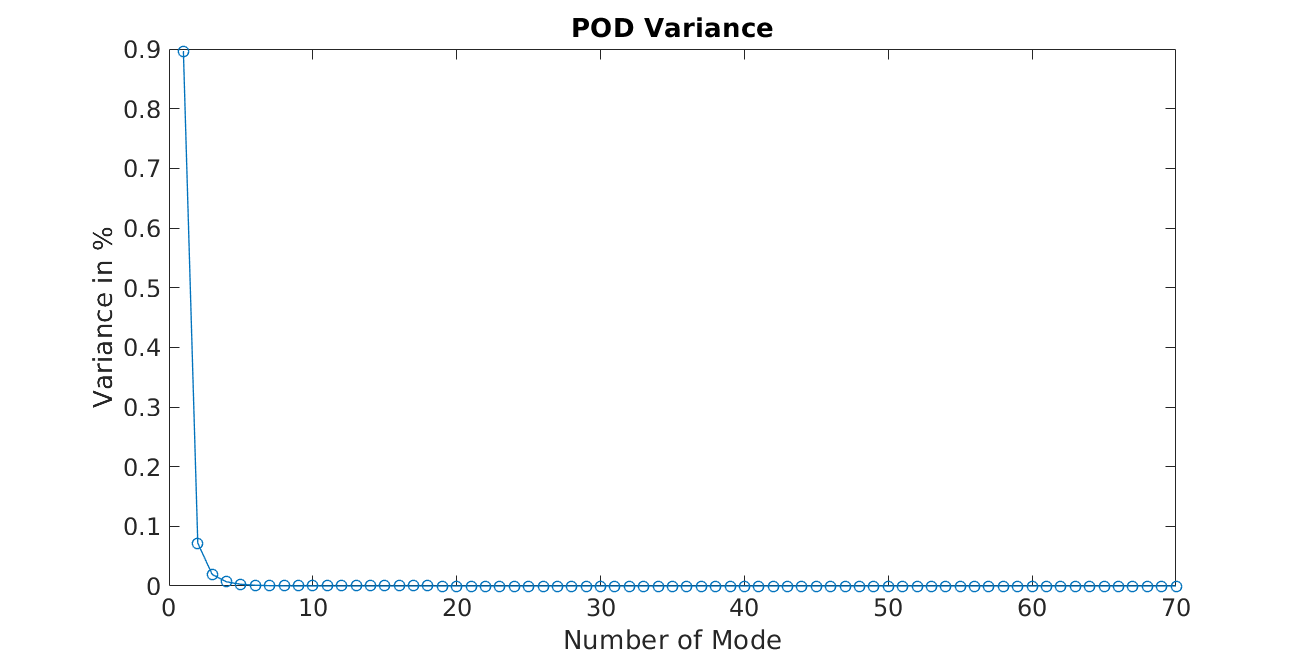
\includegraphics[ width=12.5cm]{images/pod_modes}
\caption{Variance of Modes}
\label{FIG-POD-VAR-POD}
\end{figure}
These two modes are displayed in figure \ref{FIG-POD-HIGH-MODES}.
\begin{figure}[H]
\centering
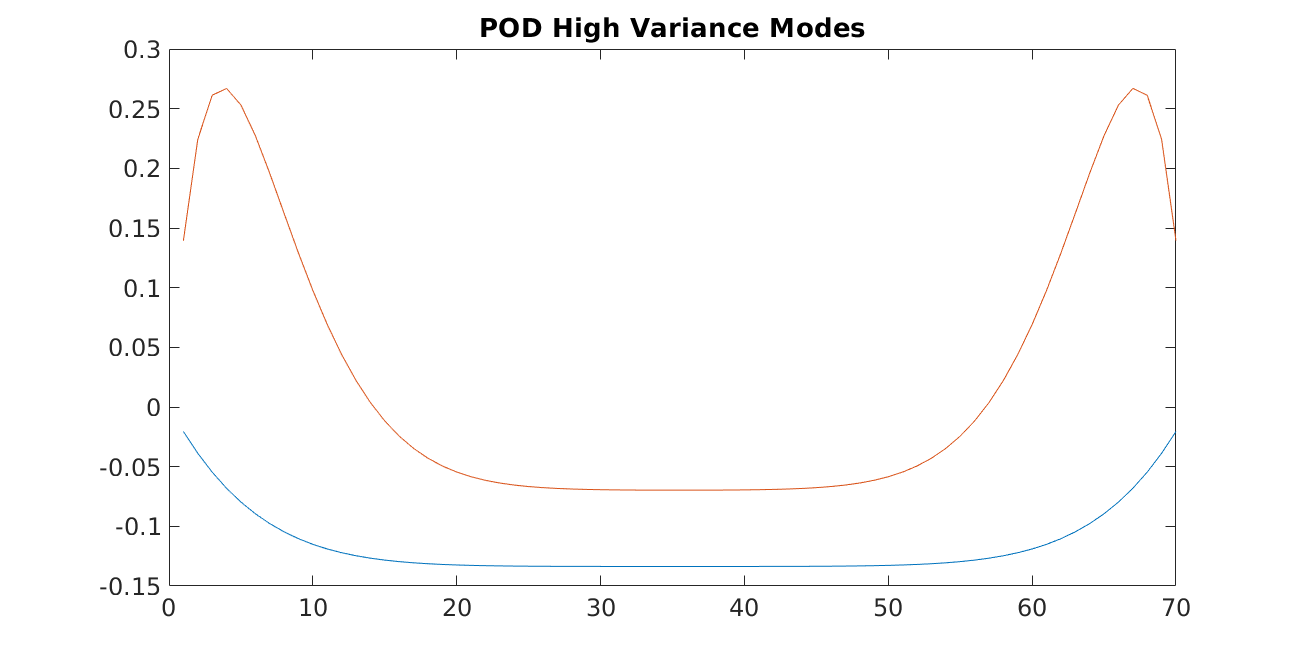
\includegraphics[ width=12.5cm]{images/pod_high_var_modes}
\caption{Leading High Variance Modes}
\label{FIG-POD-HIGH-MODES}
\end{figure}
Setting the variance too high also includes low variance modes that will introduce some errors.
Some low variance modes are displayed in figure \ref{FIG-POD-LOW-MODES}.
\begin{figure}[H]
\centering
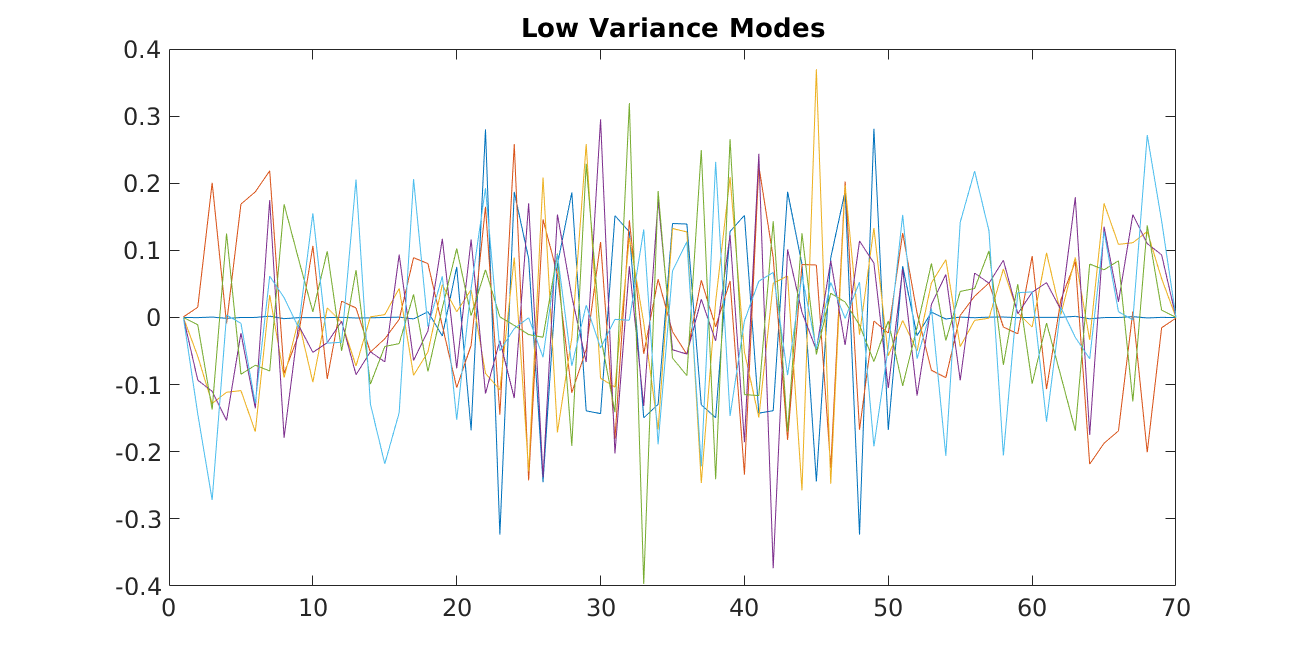
\includegraphics[ width=12.5cm]{images/pod_low_var_modes}
\caption{Modes 30 to 35}
\label{FIG-POD-LOW-MODES}
\end{figure}
Figure \ref{FIG-POD-VAR-POD} shows that modes 30 to 35 almost have zero contribution to the snapshot matrix.
Therefore including them will introduce noise to the approximation and will increase computations.
However, the benefits of this reduced order model are only relevant after the PDE has been solved once using a high dimensional system of ODEs \cite{brunton_kutz_2019c}.
\subsection{POD for Heat Equation}
In order to apply pod to the heat equation, a snapshot matrix \(X\) has to be generated.
The snapshot matrix is generated by the FEM solver described in section \ref{FEM}.
After that, \(X\) gets decomposed using the SVD.
The modes contained in \(\Phi\) are obtained by truncating the left singular vectors of \(X\) according to (\ref{PHI}).
Substituting \(\mathfrak{P}\) in (\ref{u-aprox-pod}) with heat equation \ref{eq-1d-h} results in the following
\begin{gather}
\Phi \frac{\partial a}{\partial t}  = \alpha \frac{\partial^{2} \Phi}{\partial x^{2}} a + h\\
\frac{\partial a}{\partial t} = \alpha \Phi^{T}  \frac{\partial^{2} \Phi}{\partial x^{2}} a + \Phi^{T}h \,.
\end{gather}
This system of ODEs can now be solved using Euler scheme.
Note that \(\Phi\) contains numeric values.
Therefore derivatives are unstable, especially at the first and last entries of the column vectors of \(\Phi\).
To reduce this problem, the method used to compute the second derivative of \(\Phi\) is the so-called spectral derivative.
The discrete spectral derivative works by computing the FFT of a vector.
That vector is multiplied by \((ik)^{d}\), \(d\) is the order of the derivative, and \(k\) are the discrete wave numbers.
After that step, the IFFT is applied to obtain the derivative of the original vector \cite{brunton_kutz_2019f}
\begin{gather}
f \in \mathbb{C}^{n}, \quad k = \begin{bmatrix}
\frac{n}{2} & \hdots & \frac{n}{2}
\end{bmatrix}^{T} \\
\frac{df}{dx} = \mathfrak{F}^{-1}\left\{i \frac{2 \pi k}{n} \mathfrak{F}\{f\}\right\} \\
\frac{d^{2}f}{dx^{2}} = \mathfrak{F}^{-1}\left\{-\frac{2 \pi k}{n} \mathfrak{F}\{f\}\right\} \,.
\end{gather}

Figure \ref{FIG-POD} shows a solution to heat equation using FEM and an approximation using POD with \(u(x, t) = 0, x_0 = 10000^{70\times1}, n = 70,\) variance \( = 90\%\).
The x-axis displays time in seconds, and the y-axis is the object's length.
It is visible that there are some differences, especially near the boundaries.
However, chapter \ref{analysis} covers a more detailed analysis of the error.
\begin{figure}[H]
\centering
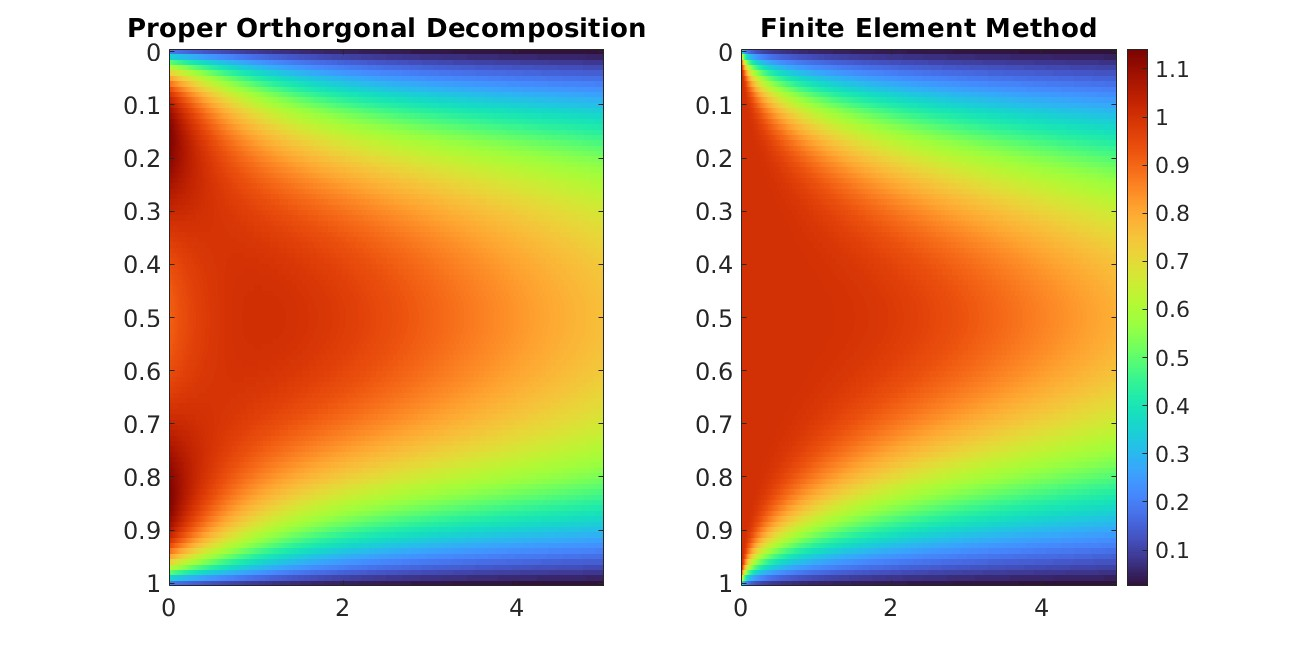
\includegraphics[ width=12.5cm]{images/pod}
\caption{FEM solution and POD approximation for heat equation}
\label{FIG-POD}
\end{figure}

